\chapter{Approach}
\label{ch:approach}
In the following section, we introduce our proposed security approach for substation automation systems.
With the aim of securing the time-critical communication between resource-constrained devices in a time-variable environment, we propose a \textbf{C}ertificateless \textbf{A}ttribute-Based \textbf{S}erver-Aided \textbf{C}ryptosystem for \textbf{S}ubstation \textbf{A}utomation \textbf{S}ystems (CASC-SAS).
The CASC-SAS cryptography and cybersecurity approach is able to prevent and mitigate cyberattacks by providing security schemes and mechanisms, and enforcing mandatory communication policies.

The introduction and discussion of the proposed approach is organized as follows.
At the beginning of this chapter in \autoref{sec:approach:system_model}, we discuss the field of application of the proposed approach by introducing a system model and defining its requirements.
Based on the presented system model and requirements, we introduce the CASC-SAS approach in \autoref{sec:approach:casc}.
The two main CASC-SAS concepts, its cryptographic scheme and server-aided access control, are introduced in \autoref{sec:approach:casa} and \autoref{sec:approach:sabaac}.
In \autoref{sec:approach:realization} we present the planned realization of the CASC-SAS approach.
Subsequently, we present the proposed evaluation strategies and metrics of the approach in \autoref{sec:approach:evaluation}.
% Finally, in \autoref{sec:approach:limitations} we discuss limitations of the proposed approach.
%\todo{Own idea, concept, protocol, evaluation, proof, testing, expected benefits and limitations}
%\todo{SECURITY: Security Goals (CIA + Privacy Preserving)}
%\todo{IDEA: Wrap packages of arbitrary protocols by encripting payload of ethernet package, and adding a new header with ABAC-SS information. Maybe as HW Middleware? If other endpoint does not support the ABAC-SS wrapping fall back to proofing endpoint via identity provider only.}
%\todo{PERF EVALUATION: 1. Run approach on network simulator, and 2. Run approach on raspberry pi's representing different roles like server, DER, user \dots}

\section{System Model}
\label{sec:approach:system_model}
In the following sections, we introduce the system model of the CASC-SAS approach.
The system model serves the purpose of delimiting the scope and area of application of the proposed approach.

The area of application of the proposed approach consists of ICSs in the power system domain.
More specifically, the proposed approach is tailored to the communication and control systems of substations in the electricity grid.
The communication and control equipment of an ICS is referred to as secondary equipment.
The entirety of secondary equipment of a substation is referred to as Substation Automation System (SAS) \cite{Padilla2015}.
Although the proposed approach is tailored to the power system domain and substation environment, its main concepts may also be applied to other ICS with similar requirements and constraints.

\subsection{Architecture}
The architecture of the presented system model is based on the IEC 61850 standard \cite{IEC61850P5}.
The presented system model architecture consists of four layers called network level, station level, bay level, and process level.
The process, bay, and station level represent the internal layers of a SAS architecture.
The SAS architecture containing the process, bay, and station level as well as the station and process bus further discussed in \autoref{sec:approach:system_model:communication} is shown in \autoref{fig:substation_architecture}.
The network level represents a SAS-external layer to integrate multiple SAS instances and supervisory controllers into a comprehensive power system.
Each of the four layers consists of different devices and provides different control and automation functions:
\begin{enumerate}
    \item Process Level: The process level provides functions to interact with the physical process via sensors and actuators.
    As a consequence, SAS devices located at the process level provide interfaces to the physical process.
    In other words, devices located at the process level transform analog measurement signals or control signals into digital values and vice versa.
    Devices restricted to the transformation and provision of measurement and control values are referred to as Merging Units (MU).
    Moreover, IEDs can be employed to combine MU functions with higher-level functions such as protection or communication tasks.

    \item Bay Level: The bay level provides common functions of so-called bays of a SAS.
    As stated by the \citeauthor{IEC61850P5} \cite{IEC61850P5}, a bay represents a closely connected subpart of a substation with common functionality.
    The devices at bay level supervise the operation of lower-level devices of a SAS bay.
    Consequently, a supervising bay level device is referred to as bay controller or bay protection.

    \item Station Level: The station level provides functions related to the substation as a whole.
    Therefore, the station level comprises devices required for on-site and remote monitoring and control of the substation.
    Devices at the station level include Human Machine Interfaces (HMI) for substation operators as well as Wide Area Network (WAN) gateways like SCADA RTUs.

    \item Network Level: The network level provides higher-level functions exceeding the scope of a single SAS.
    The network level devices include supervisory monitoring and control devices like SCADA MTUs.
\end{enumerate}
\begin{figure}
    \centering
    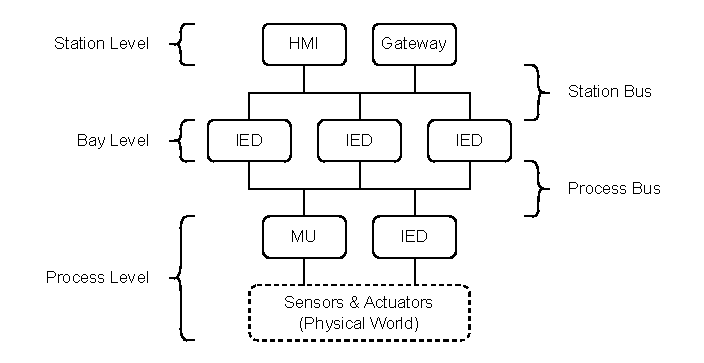
\includegraphics[width=1.0\linewidth]{figures/substation_architecture.drawio.pdf}
    % \caption{The internal SAS architecture consisting of three layers called system level, bay level, and process level which are connected via station bus and process bus.}
    \caption{Internal three-layered architecture of a SAS.}
    \label{fig:substation_architecture}
\end{figure}

\subsection{Communication}
\label{sec:approach:system_model:communication}
In the following, we discuss the communication between devices of the presented system model.
For this purpose, we identify different communication characteristics based on which communication relationships and messages can be classified.
Moreover, we define three messages types for time-critical ICS and SAS communication.
Furthermore, we discuss the bus-based device interactions occurring in the above-mentioned four layer system model.

\subsubsection{Classification Characteristics}
The communication relationships between devices can be classified using different communication characteristics.
Topological communication characteristics can be used to classify the device relationships based on their relative or absolute location within the system model.
Accordingly, communication can either occur between devices on the same layer or different layers of the system model.
Communication on the same layer of the system model is referred to as horizontal communication, whereas communication between devices on different layers is referred to as vertical communication.
Moreover, communication can occur between devices of the same or different subsystems.
Communication between devices of the same subsystem is classified as (subsystem) internal communication, whereas communication relationships including an external device are classified as (subsystem) external communication.
Furthermore, a communication relationship is not limited to a single receiver (unicast) but rather a group of devices (multicast) or all devices (broadcast) may receive a sender's message.

Besides the topology-based classification, communication relationships can be classified based on their continuity.
Continuous, session-oriented, or stateful communication requires an initial session establishment between the involved devices.
While the first message exchange requires additional initialization overhead, subsequent latencies might benefit from the established communication session.
Discontinuous, message-oriented, or stateless communication enables communication without initial overhead for the involved devices.
Consequently, discontinuous communication does not lead to latency emerging from session initialization and management.

Since communication in ICS and SAS is time-critical, communication relationships can be classified based on their communication latency constraints.
Within the scope of the proposed approach, we define communication latency as sum of processing times and transmission times required to exchange information between involved devices.
The transmission time is the time required to transmit a message over a network link with a specific throughput.
The processing time represents the time required for a device to send, forward, or receive a message or packet.
For intermediate network devices like routers and switches the processing time depends on queuing delay and forwarding delay.
For the sender and receiver of a message or packet the processing time consists of enqueue and dequeue delays, cryptographic overhead, and message coding.
As a consequence, the communication latency represents the time required for a message from being put into the sending buffer at the sender to the point when the message is taken from the receiving buffer at the receiver.

\subsubsection{Message Types}
\label{sec:approach:system_model:communication:message_types}
The defined message types of the presented system model are based on the classification characteristics defined above.
Furthermore, the defined message types have been adapted from the message types and performance classes of the IEC 61850 standard \cite{IEC61850P5}.
The defined message type as well as their typical communication topology, continuity, and latency constraints are shown in \autoref{tab:message_types}.

The low latency message type corresponds to the IEC 61850 \cite{IEC61850P5} message types 1A and 4.
The low latency messages are used for SAS-internal exchange of sampled values and state values.
In IEC 61850 compliant substations the sampled values are exchanged using the Sampled Values (SV) protocol between MUs and IEDs (vertical) or between MUs (horizontal).
Moreover, state values and state changes are exchanged horizontally between IEDs using the Generic Object Oriented Substation Events (GOOSE) protocol.

The medium latency message type corresponds to the IEC 61850 message types 1B and 2.
The medium latency messages are used for internal and external as well as horizontal and vertical session-based client-server communication.
In IEC 61850 substations IEDs use the Manufacturing Message Specification (MMS) protocol to communicate with other IEDs and higher-level devices.

The high latency message type corresponds to the IEC 61850 message types 3 and 5.
This message type is used for HMI interactions as well as non-time-critical operations like file transfers.
In IEC 61850 substations MMS as well as SCADA protocols are used for high latency communication.
\begin{table}
    \centering
    \small
    % \caption{Message types of the presented system model classified with regard to their topology, continuity, and latency constraints of the communication relationships.}
    \caption{Message types of the presented system model.}
    \label{tab:message_types}
    \begin{tabular}{l c c c c c}
    \toprule
    \multicolumn{1}{c}{Message Type} & \multicolumn{3}{c}{Topology} & Continuity & Latency\\
    & Externality & Verticality & Receiver & & Constraint\\
    \midrule
    Low Latency & Internal & Horiz./Vert. & Multicast & Message-Based & 3 ms\\
    Medium Latency & Int./Ext. & Horiz./Vert. & Unicast & Session-Based & 20-100 ms\\
    High Latency & Int./Ext. & Horiz./Vert. & Unicast & Session-Based & 500 ms\\
    \bottomrule
    \end{tabular}
\end{table}

\subsubsection{Communication Buses}
The presented system model uses a bus-based approach for SAS-internal message exchange between the system architecture layers.
The implementation of SAS-internal buses is typically based on Ethernet and open or proprietary fieldbus technology.
The bus-based approach as well as the two concrete buses introduced in the following are based on the IEC 61850 standard \cite{IEC61850P5}.

The first bus for SAS-internal message exchange is referred to as process bus.
The process bus is located between the bay level and the process level.
The process bus is used for time-critical message-based publisher-subscriber communication.
GOOSE and SV are the IEC 61850 protocols used for process bus communication.

The second bus for SAS-internal message exchange is referred to as station bus.
The station bus is located between the station level and the bay level.
The station bus connects IEDs at the bay level with each other as well as with gateways and interfaces at the station level.
The communication at the station bus is typically session-based unicast communication with less strict time requirements compared to the process bus.

SAS-external message exchange between devices on the station level and network level use WAN telecommunication technologies including Internet, satellite, cellular, and radio technology.
Secure tunneling approaches like Virtual Private Networks (VPN) can be used to enhance the security of SAS message exchange over an unsecure communication medium.

%\subsection{Threats}
%\todo{System Threats + Adversaries + Attack Trees}
\todo{Subsection: System Threats}

\subsection{Requirements}
In the following, we introduce the requirements of the presented system model.
Based on the identified requirements, functional and non-functional characteristics of the proposed approach are derived and evaluated.
Each system model requirement is associated with a requirement category.
We define five requirement categories for the introduced system requirements.
The requirement categories include security (RQ.SEC), safety (RQ.SAF), availability (RQ.AVA), performance (RQ.PER), and compatibility (RQ.COM).
\todo{Add forward/backward secrecy and more.}

\subsubsection{Security}
The system model has to satisfy six requirements related to information security.
The security requirements of the system model are defined as follows:
\begin{description}
    %\paragraph{RQ.SEC.1 Confidentiality}
    %The system prohibits unauthorized access to sensitive information stored on devices and payload of messages exchanged within the system and between systems \cite{Eckert2023}.
    \item[RQ.SEC.1] Integrity\\
    The system detects unauthorized manipulation of stored and exchanged data \cite{Eckert2023}.
    \begin{description}
        \item[RQ.SEC.1A] Device Integrity\\
        The system detects unauthorized manipulation of data that is stored on system devices.
        \item[RQ.SEC.1B] Message Integrity\\
        The system detects unauthorized manipulation of data that is exchanged between system devices.
    \end{description}
    \item[RQ.SEC.2] Authenticity\\
    The system can proof the authenticity and trustworthiness of subjects and data objects present in the system \cite{Eckert2023}.
    \item[RQ.SEC.3] Access Control\\
    The system prohibits unauthorized access to sensitive information stored on devices.
    \item[RQ.SEC.4] Non-Repudiation\\
    The system ensures that a subject cannot dispute its authorship of data and requests~\cite{Eckert2023}.
    \item[RQ.SEC.5] Principle of Least Privilege  (PoLP)\\
    The system ensures that each subject has the least number of privileges necessary to perform its function \cite{JTF2020}.
    \item[RQ.SEC.6] Separation of Duties (SoD)\\
    The system ensures that no subject has enough privileges to be able to misuse the system without collusion \cite{JTF2020}.
    %\paragraph{RQ.SEC.7 Privacy Preservation}
    %\todo{TODO: Does this conflict with the idea of proofing the origin of a request? In other words, is it possible to check if the subject who requested the access decision is still the same subject who used it in its request?}
\end{description}

\subsubsection{Safety}
The system model has to satisfy two safety-related requirements.
The safety requirements of the system model are defined as follows:
\begin{description}
    \item[RQ.SAF.1] Safe Operation\\
    Under possible operating conditions, the system must not pose a threat to itself and its environment.
    \item[RQ.SAF.2] Fail-Safe\\
    In case of failure, the system terminates without causing harm to the system or system environment~\cite{rfc4949}.
    In other words, the system never transitions into an unsafe state.
\end{description}

\subsubsection{Availability}
The system model has to satisfy two availability-related requirements.
The availability requirements of the system model are defined as follows:
\begin{description}
    \item[RQ.AVA.1] Continuing Operation\\
    Under possible operating conditions, the system must continue its operation as stated by the system requirements.
    \item[RQ.AVA.2] Fail-Operational\\
    In case of failure, the system aims to continue its operation by selectively terminating failing system functions.
    The selective termination of non-essential system functions in case of a failure is also referred to as fail-soft~\cite{rfc4949}.
\end{description}

\subsubsection{Performance}
The system model has to satisfy three requirements related to system performance.
The performance requirements of the system model are defined as follows:
\begin{description}
    \item[RQ.PER.1] Communication Latency\\
    The system must respect the latency constraints for network communication defined in \autoref{sec:approach:system_model:communication:message_types}.
    Consequently, the maximum communication latency for low latency message exchange on the data path must not exceed three milliseconds.
    \item[RQ.PER.2] Computational Complexity\\
    The system must respect the limited performance of resource-constrained devices in the SAS.
    Consequently, computationally complex algorithms have to be executed by performance-oriented servers.
    \item[RQ.PER.3] Energy \& Power Saving\\
    The system must respect the energy and power constraints of resource-constrained devices in the SAS.
\end{description}

\subsubsection{Compatibility}
The system model has to satisfy two requirements related to system compatibility.
The compatibility requirements of the system model are defined as follows:
\begin{description}
    \item[RQ.COM.1] Interoperability\\
    The system components are capable of exchanging information and providing services, irrespective of whether they originate from a single vendor or multiple vendors~\cite{IEC61850P5}.
    \item[RQ.COM.2] Interchangeability\\
    The system's behavior and functionality may not be influenced by an exchange of devices with an equal range of functions from a single vendor or multiple vendors~\cite{IEC61850P5}.
\end{description}

\section[Certificateless Attribute-Based Server-Aided Cryptosystem for SAS (CASC-SAS)]{Certificateless Attribute-Based Server-Aided Cryptosystem for Substation Automation Systems (CASC-SAS)}
\label{sec:approach:casc}
To satisfy the requirements of the above-mentioned system model, we propose a \textbf{C}ertificateless \textbf{A}ttribute-Based \textbf{S}erver-Aided \textbf{C}ryptosystem for \textbf{S}ubstation \textbf{A}utomation \textbf{S}ystems (CASC-SAS).
The CASC-SAS approach is a cryptosystem that provides security policies, cybersecurity mechanisms, and cryptographic algorithms and schemes.
The goal of the approach is the enhancement of SAS security by providing secure authentication, authorization, and attribute-based access control for time-critical SAS communication.

The CASC-SAS approach comprises two core concepts.
The first core concept of the approach is the Certificateless Attribute-Based Server-Aided Authentication (CASA).
This concept represents the foundation of the CASC-SAS approach.
The concept provides cryptographic algorithms and schemes for authentication including a public key cryptography signature scheme for key generation, signing, and verification.
Communicating SAS devices as well as more abstract cybersecurity services can rely on the provided communication integrity, authenticity, and non-repudiation.
This core concept is further discussed in \autoref{sec:approach:casa}.

The second core concept of the approach is the Server-Aided Attribute-Based Authorization and Access Control (SABAAC).
This concept provides mechanisms to enable attribute-based authorization and ABAC for time-critical SAS communication.
The concept represents a more abstract cybersecurity means to provide access control, PoLP, and SoD.
For this purpose, the concept relies on authentication services provided by CASA.
This concept is further discussed in \autoref{sec:approach:sabaac}.

\subsection{Security Architecture}
In the following, we present the security architecture of the proposed approach.
The CASC-SAS approach is based on a dual-path four-layered architecture.
The four layers of the architecture are presented in \autoref{sec:approach:casc:architecture:layers}.
Moreover, the two paths of the architecture are further discussed in \autoref{sec:approach:casc:architecture:paths}.

\subsubsection{Four-Layered Architecture}
\label{sec:approach:casc:architecture:layers}
The CASC-SAS architecture is non-strictly layered and consists of four open layers.
The goal of the layered architecture is the separation of different domains and levels of abstraction within the CASC-SAS approach.
An upper layer may use services provided by a lower layer but not vice versa.
Moreover, since the layering is non-strict, an upper layer is not restricted to the services provided by its direct predecessor, but may rather bypass lower layers.
The four layers of the CASC-SAS architecture and their provided services are defined in the following sections.

\paragraph{Layer 3: Domain}
The domain layer is the uppermost layer of the architecture.
The domain layer represents the domain-specific applications and the exchange of domain-specific messages.
We assume that the domain layer does not provide means for secure message exchange between entities.
As a consequence, the domain layer relies on the secure message exchange provided by lower layers.
%Provides insecure domain-specific messages to be exchanged between two different SAS devices\dots

\paragraph{Layer 2: Cybersecurity}
The cybersecurity layer encompasses algorithms and protocols used to satisfy the security requirements.
Additionally, security workflows and mechanisms for the enforcement of security policies are located at this layer.
Consequently, the cybersecurity layer provides secure message exchange services to the domain layer.
The SABAAC concept of CASC-SAS is part of this architectural layer.
SABAAC provides authorization and access control to satisfy the security requirements access control, PoLP, and SoD.
%Provides authorization and access control to satisfy access control, PoLP, and SoD.

\paragraph{Layer 1: Cryptography}
The cryptography layer provides cryptographic algorithms and schemes to higher layers of the architecture.
It relies on reliable and unreliable control message exchange.
The exchange of cryptographic control messages enables cryptographic workflows such as key generation, key distribution, key revocation, and server-aided cryptography.
The CASA core concept of CASC-SAS is located at the cryptography layer.
CASA provides authentication means via digital signatures to higher levels of the architecture.
Accordingly, CASA provides services that satisfy the security requirements integrity, authenticity, and non-repudiation.

\paragraph{Layer 0: Message Exchange}
The lowermost layer of the CASC-SAS architecture is referred to as message exchange layer.
The message exchange layer provides reliable and unreliable message exchange between devices in a network to higher layers.
The message exchange layer represents an abstraction of the physical layer, data link layer, network layer, and transport layer of a conventional network stack.
%Provides reliable and unreliable message exchange between devices in a network.

\paragraph{Example: Domain-Specific Communication}
\begin{figure}
    \centering
    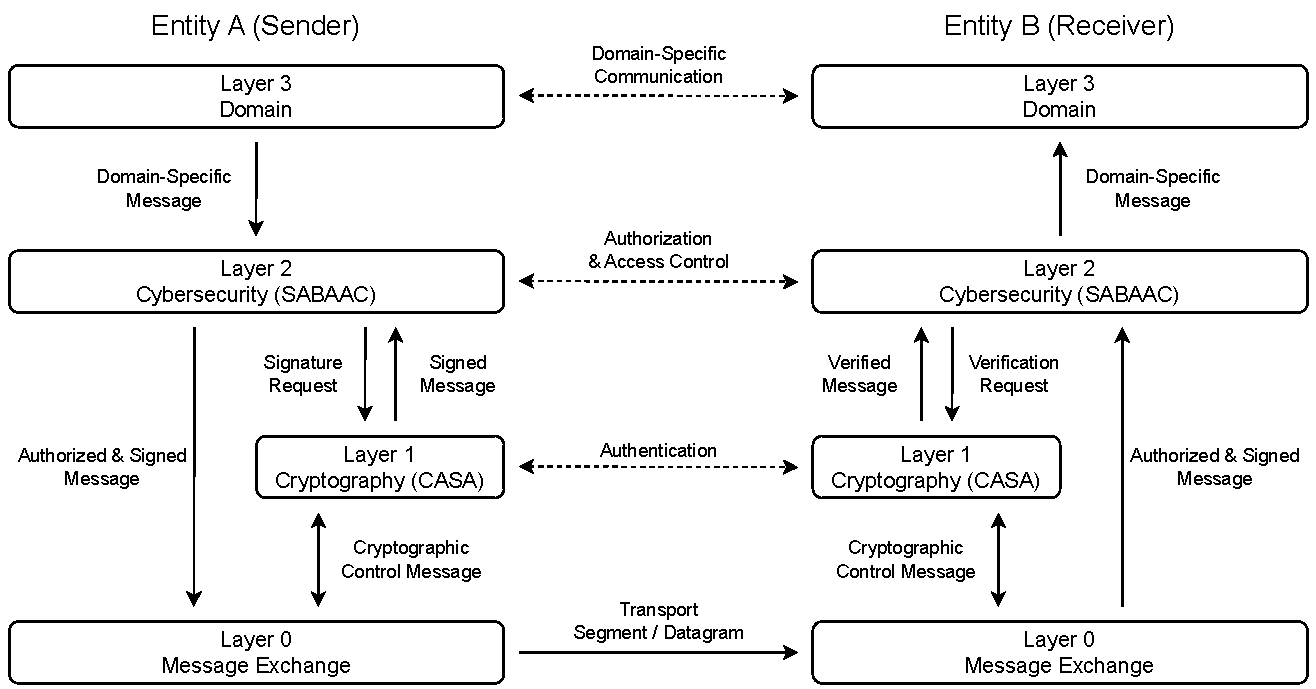
\includegraphics[width=1.0\linewidth]{figures/layers_request_example.drawio.pdf}
    % \caption{An exemplary domain-specific communication between a sending and receiving entity including the involved CASC-SAS layers and messages exchanged between the architectural layers.}
    \caption{Exemplary message exchange in four-layered CASC-SAS architecture.}
    \label{fig:layers_request_example}
\end{figure}
An exemplary domain-specific communication between a sending entity and receiving entity is shown in \autoref{fig:layers_request_example}.
The figure shows the four layers of the CASC-SAS architecture at the sender and receiver.
Moreover, the different messages exchanged between the layers are shown.
While the invocation of services is restricted to predecessor layers, message exchange resulting from an invocation may occur bidirectional.
The presented domain-specific communication is initiated by entity A.
Therefor, entity A creates a single or multiple domain-specific messages and delivers them to the cybersecurity layer.
The yet unsigned and non-authorized messages are then authorized by SABAAC and forwarded to CASA at the cryptography layer for signing.
Subsequently, the signed and authorized messages are forwarded to the receiver using the reliable and unreliable network transport services provided by the message exchange layer.
Upon arrival at the receiver, the message exchange layer delivers the signed and authorized messages to the cybersecurity layer.
The messages are then verified by the cybersecurity layer before forwarding them to the domain layer and application.
For the purpose of message verification, the cybersecurity layer enforces access control policies by verifying the validity of the message authorization.
Moreover, the message is forwarded to the cryptography layer for cryptographic verification.

\subsubsection{Dual-Path Architecture}
\label{sec:approach:casc:architecture:paths}
%Data Path (Online, time-critical communication, Domain-Specific Messages) \& Control Path (Offline, Non-Time Critical communication, CASC-SAS Messages)\dots
In addition to the separation into different layers, the occurring message exchanges within the CASC-SAS architecture are logically divided into two communication paths.
The two paths are referred to as data path and control path.

The messages on the data path are used for the forwarding of domain-specific payload from a sending entity to a receiving entity.
Besides the concrete domain-specific messages, communication required for the message forwarding are transported on the data path.
This message-related communication includes server-aided signing and verification requests as well as access control.
As a consequence, the data path is used for traffic-intensive and time-critical message exchange.

The messages on the control path are used for the exchange of management information and do not carry domain-specific payload.
The components of the CASC-SAS approach use control path messages for layer-internal communication between different devices.
The cryptography layer uses control messages for key generation, distribution, and revocation.
The cybersecurity layer uses control messages for tasks such as policy management.
As a result, the communication occurring on the control path is less traffic-intensive and less time-critical.

% \subsubsection{Stakeholders}
% \todo{Stakeholders of CASC-SAS}
\todo{Subsubsection: Stakeholders}

% \subsection{Security Policies}
% \todo{Security Policies -> Link to Requirements \& Attacks}
\todo{Subsubsection: Security Policies}

\section{Certificateless Attribute-Based Server-Aided Authentication (CASA)}
\label{sec:approach:casa}
In the following section, we present the \textbf{C}ertificateless \textbf{A}ttribute-Based \textbf{S}erver-Aided \textbf{A}uthentication (CASA) concept.
CASA is a CL-PKC approach.
The goal of CASA is to provide cryptographic algorithms and schemes for key generation, key distribution, key revocation, signing, and verification.
Moreover, the goal of CASA is to enable and support more abstract cybersecurity mechanisms like authorization and access control of the CASC-SAS approach.
Therefore, CASA represents the foundation of the employed CASC-SAS cybersecurity mechanisms.

Since CASA is a CL-PKC approach, neither certificates nor key escrow is required~\cite{AlRiyami2003}.
Moreover, the CASA approach proposes a key generation that is not only based on subject identities but rather enables public keys and private keys based on arbitrary attributes of subjects or even groups of subjects.
The key generation of the CASA approach is inspired by the alternative CL-PKC key generation technique proposed by \citeauthor{AlRiyami2003} \cite{AlRiyami2003}.
The defining characteristics of the alternative key generation is the derivation of partial private keys from public keys and identities.
As a consequence, an entity has to generate its public key before it can request a partial private key from the KGC.
This alternative key generation enables sending of partial private keys over unsecure channels and reduces the required trust in the KGC.
Furthermore, this technique allows only one public key to be created for a specific private key.

\subsection{Server-Aided Cryptography}
As PKC mechanisms may consist of computationally complex algorithms and operations such as bilinear pairing, we propose a server-aided PKC approach.
Therefor, we propose an extension of the CL-PKC concept and schemes to make time-critical steps server-aided.
To make CASA server-aided, an Untrusted Cryptography Server (UCS) supports devices by handling computationally expensive algorithms instead of executing them locally on resource-constrained devices.
To minimize the required trust, the UCS may only handle certain computations, i.e., partially sign or verify a request of a device.
This server-aided approach enables resource-constrained devices to apply secure algorithms and schemes of CASA in a time-critical OT environment.
In the following, we employ the concept of server-aided PKC for the verification process.

As stated by \citeauthor{Wu2008} \cite{Wu2008}, a server-aided verification process has to satisfy the property of being computation-saving.
A server-aided verification process $V_{Aided}$ is computation-saving if the computational costs for the verifier are strictly less than the costs of non-server-aided verification $V_{Conventional}$.
In other words, $V_{Aided}$ is computation-saving if the equation $Cost(V_{Aided}) < Cost(V_{Conventional})$ holds.

\subsection{Online \& Offline Cryptography}
Since CASA is tailored for time-critical communication, the approach aims to reduce the required time for cryptographic algorithms.
In addition to server-aided cryptography, this time reduction is achieved by precomputation.
For this purpose, each step of an algorithm is classified as either online or offline.
Online steps depend on the sender's public key, the digital signature, or the message.
Consequently, online steps cannot be precomputed.
Nevertheless, specific online steps can be accelerated via server-aided cryptography.
Offline steps depend on information that is available before any message exchange occurs.
Therefore, offline steps can be precomputed to reduce the required time for cryptographic algorithms.

\subsection{Signature Scheme $\mathcal{S}_{CASA}$}
The CASA signature scheme $\mathcal{S}_{CASA} = (I, G_{VAL}, G_{PK}, G_{PPK}, G_{SK}, S, V_{ENT}, V_{SAV}, V_{FIN})$ is a nine-tuple of algorithms.
The algorithms comprise an initialization algorithm $I$, a secret value generation algorithm $G_{VAL}$, a public key generation algorithm $G_{PK}$, a partial private key generation algorithm $G_{PPK}$, a private key generation algorithm $G_{SK}$, a signing algorithm $S$, a partial entity verification algorithm $V_{ENT}$, a partial server verification algorithm $V_{SAV}$, and a final entity verification algorithm $V_{FIN}$.
In the following sections, the specific algorithms are further discussed.

The definition of the CASA signature scheme is based on the definition of digital signature schemes provided by \citeauthor{Boneh2023} \cite{Boneh2023}.
Moreover, since CASA is a CL-PKC approach, the signature scheme has been adapted from the schemes and concepts presented by \citeauthor{AlRiyami2003} \cite{AlRiyami2003} and \citeauthor{Ramadan2023} \cite{Ramadan2023}.
The proposed server-aided verification concept and algorithms are inspired by schemes proposed by \citeauthor{Ramadan2020} \cite{Ramadan2020}, \citeauthor{Girault2005} \cite{Girault2005} and \citeauthor{Wu2008} \cite{Wu2008}.

\subsubsection{Initialization Algorithm $I$}
The initialization algorithm $(\rho, s) \leftarrow I(\lambda)$ takes the security parameter $\lambda$ as input and outputs the public system parameters $\rho$ and the private master key $s$.
The initialization algorithm is executed by the KGC.
After the execution, $\rho$ is publicly available to all entities, whereas $s$ is only known by the KGC.

\subsubsection{Secret Value Generation Algorithm $G_{VAL}$}
The secret value generation algorithm $\chi_A \leftarrow G_{VAL}(\rho)$ takes the public system parameters $\rho$ as input and outputs the secret value $\chi_A$ of an entity $A$.
The secret value generation algorithm is executed by an entity.
The secret value $\chi_A$ is never shared with other entities and may only be known to entity $A$.

\subsubsection{Public Key Generation Algorithm $G_{PK}$}
The public key generation algorithm $pk_A \leftarrow G_{PK}(\rho, \chi_A, ATT_A)$ takes the public system parameters $\rho$, the secret value of an entity $\chi_A$, and the defining attributes of entity $A$ $ATT_A$ as input.
The algorithm outputs the public verification key $pk_A$ of entity $A$.
The algorithm is executed by an entity.

\subsubsection{Partial Private Key Generation Algorithm $G_{PPK}$}
The partial private key generation algorithm $ppk_A \leftarrow G_{PPK}(\rho, s, ATT_A, pk_A)$ takes the public system parameters $\rho$, the private master key of the KGC $s$, the defining attributes of entity $A$ $ATT_A$, and the $A$'s public verification key $pk_A$ as input.
The algorithm outputs the partial private key $ppk_A$ of entity $A$.
The partial private key generation is executed by the KGC on request of an entity.
After the execution, the KGC provides the partial private key to the corresponding entity.

\subsubsection{Private Key Generation Algorithm $G_{SK}$}
The private key generation algorithm $sk_A \leftarrow G_{SK}(\rho, \chi_A, ppk_A)$ takes the public system parameters $\rho$, the secret value of an entity $\chi_A$, and the partial private key $ppk_A$ of entity $A$ as input.
The algorithm outputs the private signing key $sk_A$ of entity $A$.

\subsubsection{Signing Algorithm $S$}
The signing algorithm $\sigma \leftarrow S(sk_A, m)$ takes the private signing key $sk_A$ and message $m$ as input, and outputs the signature $\sigma$.
In other words, the signing algorithm $S$ is used by the sender $A$ of a message $m$ to generate a digital signature $\sigma$.
The generated digital signature $\sigma$ is associated with the message $m$ and the sender's private signing key $sk_A$.
\todo{Introduce Server-Aided Signing Techniques (Server-Partial-Signing, Sender-Signing) and Online/Offline Algorithm Steps.}

\subsubsection{Partial Entity Verification Algorithm $V_{ENT}$}
The partial entity verification algorithm $\sigma_{ENT} \leftarrow V_{ENT}(\rho, pk_A, m, \sigma)$ represents the first step of the server-aided verification process.
The algorithm takes the public system parameters $\rho$, the public verification key $pk_A$ of entity $A$, the message $m$, and the signature $\sigma$ as input.
The algorithm outputs the partially verified signature $\sigma_{ENT}$.
The receiver of a message executes the partial entity verification algorithm $V_{ENT}$ and sends the partially verified signature $\sigma_{ENT}$ to the UCS for server-aided verification.

\subsubsection{Partial Server Verification Algorithm $V_{SAV}$}
The partial server verification algorithm $\sigma_{SAV} \leftarrow V_{SAV}(\sigma_{ENT})$ represents the second step of the server-aided verification process.
The algorithm takes the partially verified signature $\sigma_{ENT}$ as input and outputs the partially verified signature $\sigma_{SAV}$.
The algorithm is executed by the UCS on request of a message receiving entity.
After the execution, the UCS provides the partially verified signature $\sigma_{SAV}$ to the requestor.

\subsubsection{Final Entity Verification Algorithm $V_{FIN}$}
The final entity verification algorithm $\delta \in \{accept, reject\} \leftarrow V_{FIN}(\rho, pk_A, m, \sigma, \sigma_{ENT}, \sigma_{SAV})$ represents the third and last step of the server-aided verification process.
The algorithm takes the public system parameters $\rho$, the public verification key $pk_A$ of entity $A$, the message $m$, the signature $\sigma$, and the partially verified signatures $\sigma_{ENT}$ and $\sigma_{SAV}$ as input.
The algorithm outputs the verification decision $\delta$ which is either $accept$ or $reject$.
In other words, the verification algorithm $V_{FIN}$ is used by the receiver to verify a received message $m$ sent by entity $A$ based on an appended signature $\sigma$.
As $\sigma$ is associated with the message $m$ and the sender's private signing key $sk_A$, it allows the receiver to verify the integrity and authenticity of the received message $m$ using the sender's public verification key $pk_A$.

\subsection{Security Model}
The proposed signature scheme $\mathcal{S}_{CASA}$ is a secure signature scheme if it is existentially unforgeable under an adaptive chosen-message attack (EUF-CMA)~\cite{Boneh2023, Goldwasser1988}.
To create an existential forgery, i.e., output a valid pair of message and signature for a new message, an adversary carrying out a CMA can request valid signatures from an entity for any message of his choice.
While non-adaptive CMA restricts the adversary to a fixed set of messages chosen prior to the attack, adaptive CMA allows the adversary to request signatures of messages depending on previously obtained signatures.
% \citeauthor{Goldwasser1988} describe an adaptive CMA as most powerful attack possible for an enemy restricted to using the signature scheme.

\section{Server-Aided Attribute-Based Authorization \& Access Control (SABAAC)}
\label{sec:approach:sabaac}
The second core concept of the CASC-SAS approach is the \textbf{S}erver-Aided \textbf{A}ttribute-\textbf{B}ased \textbf{A}uthorization and \textbf{A}ccess \textbf{C}ontrol (SABAAC).
The SABAAC approach enables the employment of attribute-based authorization and access control for time-critical SAS communication.
Therefore, the approach prevents unauthorized access and extraction of information.
The approach enables CASC-SAS to satisfy the access control, PoLP, and SoD security requirements.
Moreover, the expressive and flexible but yet computationally expensive ABAC policies are handled in a server-aided manner to satisfy the strict time constraints of the SAS domain.

Our authorization and access control approach represents a cybersecurity concept that is located on the cybersecurity layer of the CASC-SAS architecture.
Since the approach is located on the cybersecurity layer, it relies on secure authentication services provided by CASA.
As a consequence, the approach assumes that efficient and secure signing and verification algorithms are available.
In other words, CASA provides secure cryptographic algorithms and schemes that enable SABAAC to realize secure authorization and access control.

The proposed authorization and access control approach is based on a function-oriented component-based architecture.
The architecture and components are further discussed in \autoref{sec:approach:sabaac:architecture}.
Furthermore, the approach is divided into two central tasks or protocols.
The first task is referred to as delegated attribute-based authorization.
The delegated attribute-based authorization is responsible for the access control policy creation, management, storage, and distribution.
This process partially takes place prior to occurring access requests and corresponding access decisions.
The delegated attribute-based authorization protocol is further discussed in \autoref{sec:approach:sabaac:authorization}.
The second central task is referred to as delegated ABAC.
The delegated ABAC is responsible for the policy decision exchange and policy enforcement.
This process takes place when an entity initiates the communication with another entity.
The delegated ABAC protocol is further discussed in \autoref{sec:approach:sabaac:accesscontrol}.
An overview of the SABAAC architecture, components, and protocols as well as the integration of CASA components and services into the SABAAC approach are shown in \autoref{fig:sabaac_protocols_overview}.
\begin{figure}
    \centering
    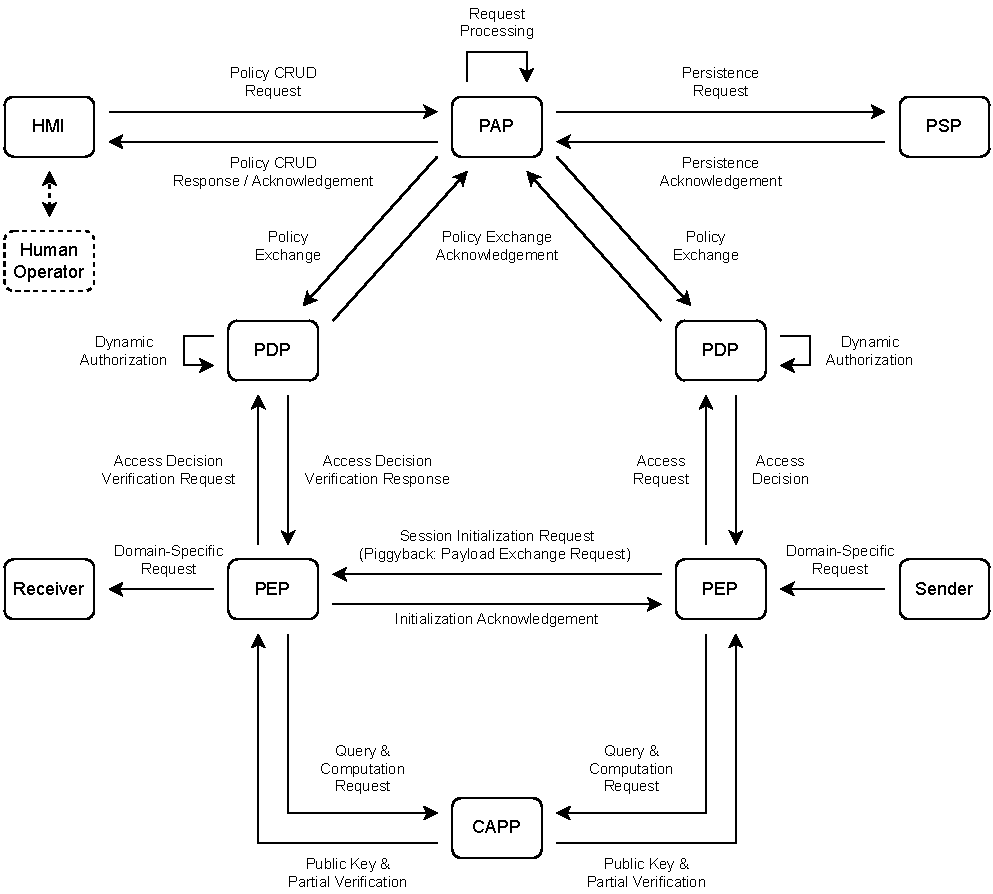
\includegraphics[width=1.0\linewidth]{figures/SABAAC_protocols_overview.drawio.pdf}
    % \caption{Component-based architecture and communication protocols of the SABAAC approach, including the four SABAAC components, their interrelationships, and the integration of CASA components and services into the authorization and access control workflow.}
    \caption{Function-oriented component-based architecture of the SABAAC approach.}
    \label{fig:sabaac_protocols_overview}
\end{figure}

\subsection{Authorization \& Access Control Architecture}
\label{sec:approach:sabaac:architecture}
The component-based architecture of our authorization and access control approach consists of four functional units.
These functional units have been adapted from the access control mechanism functional points presented by \citeauthor{Hu2014} \cite{Hu2014}.
Each functional unit is represented by a component that offers function-oriented services.
The components of the architecture are TTPs since the semantic validity of their provided services is not verifiable by the service consumers.
We specify the components as semi-trusted for the access control problem due to the restriction to access control tasks and available mitigation approaches such as multiple instances of a single component.
The four components of the architecture are discussed in the following:
\begin{description}
    \item[Policy Administration Point (PAP)] The PAP offers services for the policy creation, management, and distribution.
    The PAP is a component of the delegated attribute-based authorization process and executes the corresponding authorization protocols.
    Moreover, it provides interfaces for policy management services to human operators.
    The PAP accesses the PSP to persist policies and policy changes.
    \item[Policy Storage Point (PSP)] The PSP acts as a repository to make created policies and changes to policies persistent.
    Therefor, the PSP offers Create, Read, Update, and Delete (CRUD) services to PAP instances.
    The physical PSP instance may be integrated with the PAP component to avoid network communication overhead.
    \item[Policy Decision Point (PDP)] The PDP takes access control decisions by evaluating policies.
    The PDP takes decision on request of a PEP and provides the access control decision to the requesting PEP.
    As a consequence, the PDP is part of the delegated ABAC task of SABAAC.
    Furthermore, in the SABAAC architecture the PDP incorporates the services provided by the context handler which was introduced by \citeauthor{Hu2014} \cite{Hu2014}.
    Therefore, the PDP not only takes access control decision on request but is rather responsible for the policy and attribute evaluation workflow.
    This workflow includes the retrieval of required attributes and speedup techniques such as access decision caching and policy evaluation precomputation.
    \item[Policy Enforcement Point (PEP)] The PEP enforces access control decisions by controlling access to protected objects.
    As a consequence, the PEP is part of the delegated ABAC task of SABAAC.
    The services provided by the PEP rely on access control decisions taken by the PDP.
    % To reduce the required trust in the PDP decision, the PEP can query multiple PDPs to validate the access control decision taken.
    Moreover, in the SABAAC architecture the PEP incorporates the services provided by the Policy Information Point (PIP) introduced by \citeauthor{Hu2014} \cite{Hu2014}.
    Accordingly, the SABAAC PEP provides attributes related to its protected objects to the PDP.
\end{description}

\subsection{Access Control Policy}
\label{sec:approach:sabaac:policy}
According to \citeauthor{Hu2014} \cite{Hu2014}, ABAC is an access control model that enables access decisions based on attributes associated with subjects, objects, actions, and the environment of a system.
An ABAC policy represents a set of rules that describe under which environmental conditions a certain subject is granted to perform certain actions on a specific protected object.

The SABAAC approach relies on the concept of attribute-based policies and access control due to the following benefits:
ABAC enables multifactor policy expression, while RBAC and IBAC limit the policy expressiveness by only relying on either roles or identities.
Consequently, the multifactor policy expression enables fine-grained and flexible access control.
Moreover, as stated by \citeauthor{Hu2014} \cite{Hu2014}, the use of ABAC can avoid explicit authorizations prior to a request.
In other words, an ABAC policy can be dynamically evaluated at the time of a request.
This dynamic evaluation allows the use of attributes from a time-variable environment.
As stated by \citeauthor{Burmester2013} \cite{Burmester2013}, a real-time attribute represents an attribute whose value is time-dependent.
Given an attribute evaluation function $E_{ATT}$ and a point of time $t$, the value $\lambda_a$ of a real-time attribute $a$ is defined by $E_{ATT}(a, t) = \lambda_a$.
To handle policies based on their degree of time-variability, the SABAAC approach classifies policies as follows:
\begin{description}
    \item[Dynamic Policy] A dynamic policy $\rho$ is an ABAC policy whose evaluation relies on at least one time-variable subject, object, environment, or action attribute.
    A policy $\rho$ is dynamic iff $\exists a \in \rho: \exists t_i \neq t_j: E(a,t_i) \neq E(a,t_j)$.
    Due to the time-variable evaluation of dynamic policies, access decisions must have a limited time of validity that corresponds to the change rate of the underlying attribute values.
    As a result, caching of access decisions that are based on dynamic policies should be avoided.
    A dynamic policy is also referred to as real-time policy.
    \item[Static Policy] A static policy $\rho$ is an ABAC policy whose evaluation does not rely on time-variable subject, object, environment, or action attributes.
    A policy $\rho$ is static iff $\forall a \in \rho: \forall t_i,t_j: E(a,t_i) = E(a,t_j)$.
    Since static policies do not rely on time-variable attributes, access decisions can be cached.
    Moreover, due to the non-frequent attribute retrieval and evaluation as well as access decision caching, static policies are a viable solution for low latency message exchange.
    A static policy is also referred to as non-real-time policy.
\end{description}
\todo{Policy DSL}

\subsection{Delegated Attribute-Based Authorization Protocol}
\label{sec:approach:sabaac:authorization}
In the following, we discuss the delegated attribute-based authorization protocol of the SABAAC approach.
Authorization is the process of assigning access privileges for protected objects to subjects \cite{Eckert2023}.
According to \citeauthor{Eckert2023} \cite{Eckert2023}, a subject is said to be authorized for a specific request if it has the required access privileges for the request.
We propose an authorization protocol that is responsible for the policy creation, management, storage, and distribution.
For this purpose, the authorization protocol provides policy management services for human operators at the PAP.
Moreover, the authorization protocol provides services for the exchange of policies between the PAP, PSP, and PDP.

The delegated attribute-based authorization protocol is a message-based protocol.
It uses digital signatures and verification provided by CASA to verify the integrity and authenticity of messages.
Moreover, the services provided by the authorization protocol use reliable and acknowledged transport layer protocols for the message exchange.
Since the authorization protocol is delegated, authorizations are not managed by the protected devices, but management is rather delegated to a TTP.
In the SABAAC approach this TTP is represented by the PAP, PSP, and PDP.
Accordingly, the protected objects or devices delegate the authorization process to these SABAAC components.
Therefore, the authorization can also be referred to as server-aided authorization.

Since no cybersecurity layer sessions are established and consequently neither nonces nor sequence numbers can be used, message exchange of the authorization protocol is vulnerable to replay attacks.
Therefore, we propose using timestamp-based replay protection for authorization messages.
At the sender, timestamp-based replay protection can be achieved by adding a timestamp to the message and digitally signing the message and timestamp together.
The message is then sent over the network to the receiver.
The receiver only processes the message payload if its timestamp has a reasonable deviation from the current time.
Moreover, if the receiver keeps record of the last timestamp received from each sender, the receiver can acknowledge duplicated and older packets without processing them.

Authorizations in the SABAAC approach are realized using ABAC policies.
As discussed in \autoref{sec:approach:sabaac:policy}, access control policies are classified as either static or dynamic.
Consequently, the authorization protocol has to take the time-variability into account.
For this purpose, the authorization protocol consists of three parts or sub-protocols:
\begin{description}
    \item[Static Authorization] The static authorization process is responsible for the creation, modification, and deletion of policies.
    The static authorization is initiated by a human operator.
    The human operator sends a policy creation, modification, or deletion request to a PAP.
    The PAP then translates the request into a valid SABAAC policy or policy modification and sends it to the PSP in the form of a CRUD request.
    Finally, the PSP persists the created or modified policy and sends a response to the PAP.
    The static authorization process, the involved components, and the occurring message exchanges are visualized in \autoref{fig:sabaac_authorization_static}.
    \begin{figure}
        \centering
        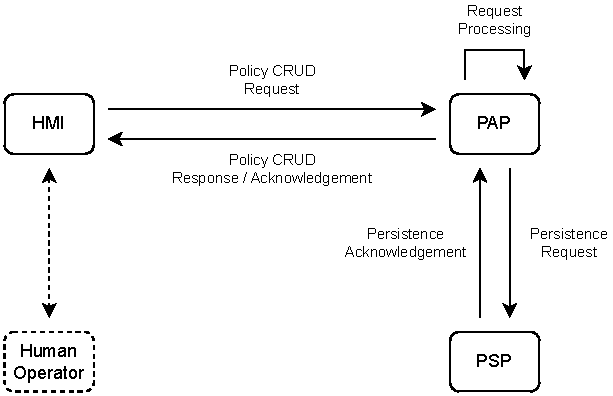
\includegraphics[width=0.9\linewidth]{figures/SABAAC_protocols_authorization_static.drawio.pdf}
        \caption{Exchanged messages of the static authorization process.
        % The process is initiated by a policy modification request of a human operator at a HMI. The involved PAP instance relies on a PSP to persist static authorizations or SABAAC policies. Requests to persist changes to static authorizations are communicated in the form of CRUD requests between the PAP and PSP.
        }
        \label{fig:sabaac_authorization_static}
    \end{figure}
    \item[Policy Exchange] After a policy is created or modified via static authorization, it is shared with the PDPs via policy exchange.
    The policy exchange is an interaction between a PAP and a PDP either initiated by a static authorization or on request of the involved PDP.
    The static authorization is a prerequisite for both policy exchange procedures.
    The policy exchange is a prerequisite for dynamic authorization at a PDP.
    A repeatedly executed dynamic authorization process may be initially triggered by a policy exchange.

    In the event that a static authorization triggers the policy exchange, the PAP sends a policy exchange message to a PDP, which contains the newly created or modified policy.
    This type of policy exchange is an incremental process.
    Consequently, only newly created or modified policies are exchanged.
    The incremental policy exchange is shown in \autoref{fig:sabaac_authorization_dynamic_policyexchange_incremental}.

    A policy exchange containing all relevant policies can be initiated by a PDP by sending a policy exchange request to a PAP.
    This type of policy exchange is referred to as complete policy exchange.
    The complete policy exchange is shown in \autoref{fig:sabaac_authorization_dynamic_policyexchange_complete}.
    \begin{figure}
        \centering
        \begin{subfigure}[t]{0.48\linewidth}
            \centering
            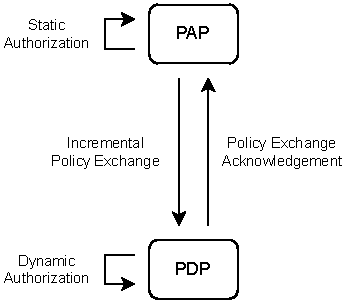
\includegraphics[width=\linewidth]{figures/SABAAC_protocols_authorization_dynamic_policyexchange_incremental.drawio.pdf}
            \caption{Incremental policy exchange procedure initiated by the static authorization of a PAP.}
            \label{fig:sabaac_authorization_dynamic_policyexchange_incremental}
        \end{subfigure}
        \hfill
        \begin{subfigure}[t]{0.48\linewidth}
            \centering
            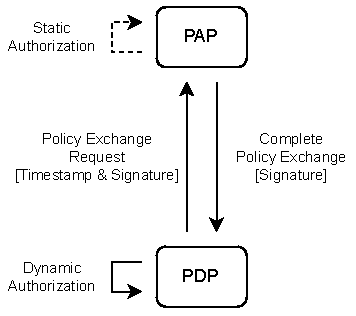
\includegraphics[width=\linewidth]{figures/SABAAC_protocols_authorization_dynamic_policyexchange_complete.drawio.pdf}
            \caption{Complete policy exchange procedure initiated by a policy exchange request of a PDP.}
            \label{fig:sabaac_authorization_dynamic_policyexchange_complete}
        \end{subfigure}
        \caption{Exchanged messages of the policy exchange procedures.
        %The static authorization is a prerequisite for both policy exchange procedures. The policy exchange is an interaction between a PAP and a PDP either initiated by a static authorization or on request of the involved PDP. The policy exchange is a prerequisite for dynamic authorization at a PDP. A repeatedly executed dynamic authorization process may be initially triggered by a policy exchange.
        }
        \label{fig:sabaac_authorization_dynamic_policyexchange}
    \end{figure}
    \item[Dynamic Authorization] The dynamic authorization process is responsible for the evaluation of SABAAC policies.
    The dynamic authorization process is executed by the PDP.
    The goal of the process is to compute whether a certain subject is authorized for a specific request.
    Therefor, the PDP retrieves the attributes related to a policy and derives an access decision.
    The dynamic authorization is either executed ad-hoc to respond to an access control request or executed prior to a request.
    The former execution strategy has less management overhead, since it requires no caching of policy evaluations.
    On the contrary, ad-hoc policy evaluation increases the response time for access control requests.
    The latter execution strategy evaluates policies prior to a request and caches the corresponding access decision.
    Consequently, this precomputation strategy enables low latency communication by reducing the response time for access control requests.
\end{description}

\subsection{Delegated Attribute-Based Access Control Protocol}
\label{sec:approach:sabaac:accesscontrol}
%\todo{Server-Aided ABAC is Delegated ABAC, Distributed Evaluation Strategy (With PDP, Ad-Hoc, Time Variable Attributes), Requests(External, Internal), Protocols, Session-Based via OAT (Estab. channel before comm.), Multiple PDPs and voting due to semi-trusted}
%\paragraph{Unicast: Client-Server Protocol}
%\paragraph{Multicast \& Broadcast: Publisher-Subscriber Protocol}
In the following, we discuss the delegated attribute-based access control protocol of the SABAAC approach.
The goal of the access control protocol is the exchange and enforcement of access control decisions.
The access control decisions are derived from the dynamic authorization process discussed in \autoref{sec:approach:sabaac:authorization}.
Since the PDP instances execute the dynamic authorization process, the provisioning of access decisions is delegated to the PDP instances as well.
In other words, the PDP instances compute access decision using dynamic authorization and provide these decisions to devices using the access control protocol.
Moreover, devices including requesting subjects and protected objects delegate the enforcement of access decisions to trusted PEP instances.

The access control protocol of the SABAAC approach uses digitally signed and partially acknowledged message exchange.
Similar to the authorization protocol, it uses digital signatures and verification provided by CASA to verify the integrity and authenticity of messages.
To exchange messages on the control path, the access control protocol relies on reliable transport services provided by the message exchange layer.
Data path message exchange of the access control protocol relies on either reliable or unreliable transport services depending on requirements such as message integrity and congestion tolerance.
Moreover, the protocol is based on discontinuous message-based communication as well as continuous session-based communication at the cybersecurity layer.
The access control sessions are initialized at the sending and receiving entities prior to the exchange of domain-specific messages.

The security of the access control protocol is vulnerable to three distinct threats.
Due to its communication architecture the protocol is vulnerable to replay, Denial-of-Service (DoS), and collusion attacks.
Replay of messages represents a threat for session-based and message-based communication.
Session-based communication of the protocol uses session identifiers and sequence numbers to provide replay protection.
Message-based communication employs timestamp-based replay protection, similar to the discontinuous communication used by the authorization protocol.
DoS attacks represent a threat for session-based communication due its stateful concept including session initialization and management.
To mitigate malicious DoS attacks and DoS due to configuration and system errors, the access control uses a soft-state session-based message exchange.
Accordingly, the session states used by the communicating entities have to be refreshed periodically and unused or invalid states are deleted.
As a consequence, devices may not make assumptions about the current state of other devices.
Moreover, a device has to handle session state exceptions via reinitialization of access control sessions.
The third type of security threat is the collusion of malicious PDP and PEP instances.
A collusion attack occurs if a PDP forges an access decision that is used by a PEP to access a protected object in an unauthorized manner.
To mitigate collusion and reduce the trust in a PDP, a PEP can use server-aided access decision verification.
Therefor, a PEP can request the verification of a PDP access decision from another PDP.

The workflow of the access control protocol is divided into three mandatory phases and an optional verification phase.
The phases of the access control protocol are defined as follows:
\begin{description}
    \item[Access Request] The access request represents the initial phase of the access control procedure.
    The goal of the access request phase is to exchange an access decision between a PDP and PEP.
    The access request phase is initiated by a PEP instance on behalf of a domain subject.
    Therefor, the PEP sends an access request including a digital signature and timestamp to a PDP.
    The PDP verifies the request based on the signature and timestamp.
    The PDP then derives an access decision from the access request and the dynamic authorization process.
    The access decision can either grant or deny the requested access.
    Finally, the signed access decision is returned to the requesting PEP.
    A PEP instance can either initiate the access request ad-hoc as soon as a domain request arrives or execute the access request prior to an arriving domain request.
    The latter option reduces the time before domain-specific payload can be transmitted to the receiving devices.

    To take the time-variability of access control policies into account, the exchanged access decision has to contain a period of validity.
    As long as an access decision is valid, it can be cached and reused by the PEPs.
    Moreover, the access decision has to contain parameters to uniquely identify the access request.
    These request parameters are used at the sending and receiving PEPs to identify the access control session.
    Since arbitrary header-specific and payload-specific information can be used for session identification, the SABAAC approach defines the mandatory identification parameters.
    Domain-specific message exchange that is based on data link layer protocols such as Ethernet is at least identified by a triple of parameters.
    The identifying triple consists of source address, destination address, and communication protocol.
    Domain-specific message exchange that is based on transport layer protocols such as the Transmission Control Protocol (TCP) or the User Datagram Protocol (UDP) is at least identified by a five-tuple of parameters.
    The identifying five-tuple consists of source address, source port, destination address, destination port, and communication protocol.
    \item[Session Initialization] The session initialization is executed by a PEP instance that is granted access via access request phase.
    To initialize an access control session, a PEP sends a session initialization request to another PEP.
    The digitally signed request has to contain a PDP-signed granted access decision and an initial sequence number.
    Moreover, the PEP may send the initialization request along with a domain-specific request by piggybacking a payload exchange request.
    A more detailed examination of the piggybacking approach is provided below.
    On receipt of an initialization request, a PEP verifies the signature of the request, the signature of the access decision, and its period of validity.
    The PEP may optionally use server-aided access decision verification that is further discussed in the following section.
    If the received request is valid, the PEP initializes a session state, sends a positive initialization acknowledgement to the requestor, and starts processing piggybacked domain-specific requests.
    If the request is invalid, the PEP sends a negative initialization acknowledgement to the requestor and discards the piggybacked domain-specific request.

    A successful session initialization between two PEPs is shown in \autoref{fig:sabaac_accesscontrol_initialization}.
    Besides the session initialization procedure, the figure visualizes a preceding access request.
    The access request procedure relies on an interaction between a PDP and a PEP and is a prerequisite for the session initialization.
    As illustrated in the figure, the session initialization relies on an interaction between two PEP instances.
    Moreover, a server-aided access decision verification at the receiving PEP is shown.
    The receiver's PEP uses a server-aided access decision verification provided by a PDP to reduce the trust in another PDP.
    Additionally, the shown SABAAC components, especially resource-constrained PEP instances, rely on the services provided by a CASA UCS for SAV.
    \begin{figure}
        \centering
        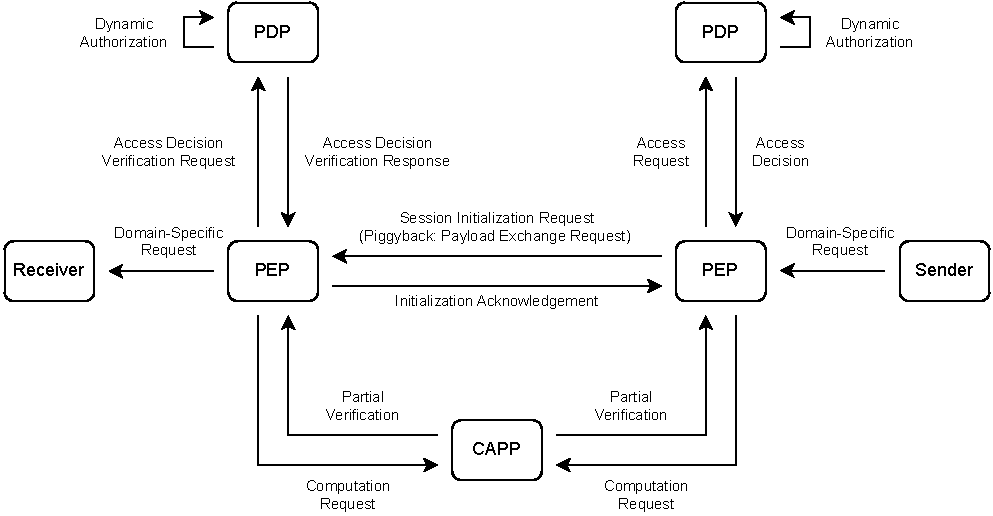
\includegraphics[width=1.0\linewidth]{figures/SABAAC_protocols_accesscontrol_initialization.drawio.pdf}
        \caption{Exchanged messages of an access request, unidirectional session initialization, and access decision verification.
        % The access request procedure relies on an interaction between a PDP and a PEP and is a prerequisite for the session initialization. The session initialization relies on an interaction between two PEP instances. The receiver's PEP uses a server-aided access decision verification provided by a PDP to reduce the trust in another PDP. The shown SABAAC components, especially resource-constrained PEP instances, rely on the services provided by a CASA UCS for SAV.
        }
        \label{fig:sabaac_accesscontrol_initialization}
    \end{figure}
    \item[Access Decision Verification] The optional server-aided access decision verification enables a PEP to verify received access decisions.
    Therefor, the PEP sends a verification request containing the PDP-signed access decision to another PDP.
    The PDP verifies the access decision and sends a positive or negative verification acknowledgement back to the requestor.
    \item[Payload Exchange] The payload exchange phase is the final phase of the access control protocol.
    This phase can be repeatedly executed until the period of validity of an underlying access control session ends.
    The goal of the payload exchange phase is to securely exchange domain-specific requests between a sender and a receiver by employing authentication, authorization, and access control mechanisms.
    The payload exchange is initiated by a domain entity via delivery of a domain-specific request to its PEP.
    On receipt of a domain-specific request, the sender's PEP appends a valid session-specific sequence number to the request.
    This extended request is then digitally signed and sent to the receiver's PEP.
    On receipt of the extended request, the receiving PEP derives the session identifying parameters from the request.
    Based on these parameters, the PEP verifies that a valid access control session for the received domain-specific request exists.
    Moreover, the PEP verifies the sequence number and signature of the extended message.
    If the received extended request is valid, the receiving PEP extracts the domain-specific request and delivers it to the corresponding domain entity.

    A successful unidirectional payload exchange between a sender and receiver is shown in \autoref{fig:sabaac_accesscontrol_payloadexchange}.
    The shown procedure relies solely on the interaction of PEP instances, with the exception of a single server-aided CASA verification on message receipt.
    \begin{figure}
        \centering
        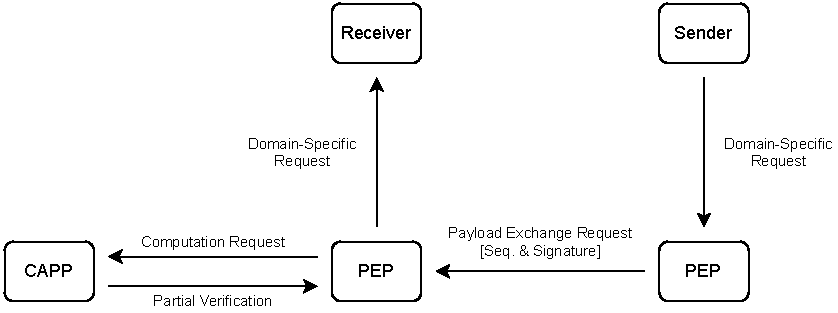
\includegraphics[width=1.0\linewidth]{figures/SABAAC_protocols_accesscontrol_payloadexchange.drawio.pdf}
        \caption{Exchanged messages of a unidirectional payload exchange procedure.
        % The procedure relies solely on the interaction of PEP instances, with the exception of a single server-aided CASA verification on message receipt.
        }
        \label{fig:sabaac_accesscontrol_payloadexchange}
    \end{figure}
    
    Domain-specific communication is unidirectionally handled by the access control protocol of SABAAC.
    Consequently, a response to a domain-specific request is handled as independent message exchange by the PEPs.
    Moreover, the payload exchange phase relies on a Negative Acknowledgement (NACK) concept
    A NACK is sent in case of verification or authorization exceptions.
    The NACK concept avoids acknowledgement implosions in multicast and broadcast communication scenarios.
    A received NACK may trigger a session reinitialization workflow at a PEP.

    To reduce the overhead of session initialization handshaking, the requesting PEP may send the session initialization request along with a domain-specific request by piggybacking a payload exchange request.
    The processing of piggybacked payload exchange requests starts as soon as the received initialization request is successfully verified.
    If an initialization request is invalid, the PEP discards the piggybacked payload exchange request.
    The usage of piggybacking decreases the required time until a domain-specific request arrives at a PEP if no session was initiated prior to the request.
    Since session initialization requires at least one RTT for handshaking, a non-piggybacked domain-specific request is delayed by at least one RTT.
    Moreover, due to the reason that session initialization is handled unidirectionally, handshaking leads to at least two RTT delay for bidirectional domain-specific communication.

    A simplified session initialization procedure between two PEP instances is visualized in \autoref{fig:sabaac_accesscontrol_initialization_rtt}.
    For RTT comparison purposes, the semantically identical session initialization handshakes and message exchanges are shown without and with piggybacking of payload exchange requests.
    A session initialization procedure without piggybacking is shown in \autoref{fig:sabaac_accesscontrol_initialization_rtt_nopiggyback}, whereas \autoref{fig:sabaac_accesscontrol_initialization_rtt_piggyback} visualizes the semantically identical procedure using piggybacked requests.
    As shown in \autoref{fig:sabaac_accesscontrol_initialization_rtt_nopiggyback}, three RTTs are the minimum time until a response to a domain-specific request can be received if no piggybacking is used.
    This three RTT delay consists of one RTT for forward session initialization, a half RTT for the forward payload exchange request, one RTT for backward session initialization, and a half RTT for the backward payload exchange request.
    %The usage of piggybacking decreases the minimum time until a response is received to a single RTT.
    The use of piggybacking reduces the minimum time required to deliver the first payload exchange request from two RTTs to a half RTT under the assumption of symmetric transmission times.
    The minimum time until a response is delivered for the initial payload exchange request is reduced from three RTTs to a single RTT.
    After the bidirectional initialization of sessions, the minimum time required for a bidirectional payload exchange equals one RTT for both scenarios.
    \begin{figure}
        \centering
        \begin{subfigure}[t]{0.48\linewidth}
            \centering
            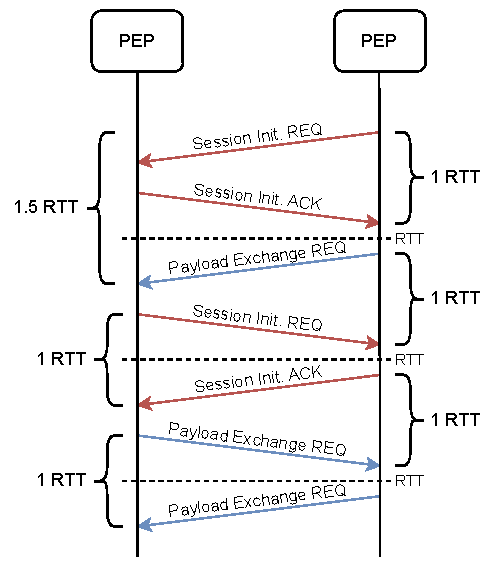
\includegraphics[width=\linewidth]{figures/SABAAC_protocols_accesscontrol_initialization_rtt_nopiggyback.drawio.pdf}
            \caption{Bidirectional session initialization and payload exchange without piggybacking.}
            \label{fig:sabaac_accesscontrol_initialization_rtt_nopiggyback}
        \end{subfigure}
        \hfill
        \begin{subfigure}[t]{0.48\linewidth}
            \centering
            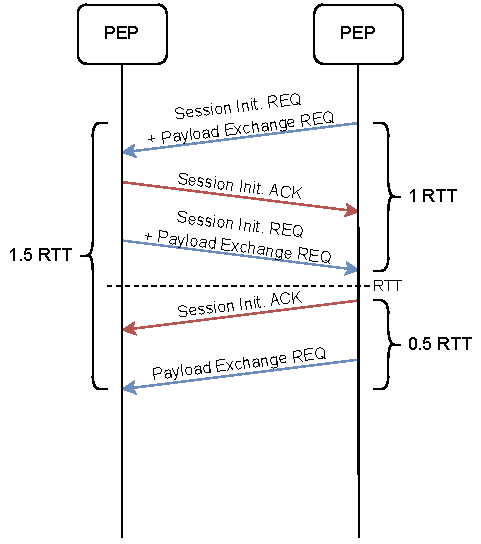
\includegraphics[width=\linewidth]{figures/SABAAC_protocols_accesscontrol_initialization_rtt_piggyback.drawio.pdf}
            \caption{Bidirectional session initialization and payload exchange with piggybacking.}
            \label{fig:sabaac_accesscontrol_initialization_rtt_piggyback}
        \end{subfigure}
        \caption{Protocol sequence diagrams of bidirectional session initialization and message exchange.
        % Protocol sequence diagrams showing a simplified piggybacking and non-piggybacking initialization of sessions for bidirectional message exchange and payload exchange between two PEP instances. For RTT comparison purposes, the semantically identical session initialization handshakes and message exchanges are shown without and with piggybacking of payload exchange requests. The use of piggybacking reduces the minimum time required to deliver the first payload exchange request from two RTTs to a half RTT under the assumption of symmetric transmission times. The minimum time until a response is delivered for the initial payload exchange request is reduced from three RTTs to a single RTT. After the bidirectional initialization of sessions, the minimum time required for a bidirectional payload exchange equals one RTT for both scenarios.
        }
        \label{fig:sabaac_accesscontrol_initialization_rtt}
    \end{figure}
\end{description}

\section{Realization}
\label{sec:approach:realization}
In the following section, we discuss the proposed realization of the CASC-SAS approach and its two core concepts CASA and SABAAC.
The approach and its two concepts introduce components that are defined and discussed in \autoref{sec:approach:casa} and \autoref{sec:approach:sabaac}.
% These components have to be integrated into the SAS system model to employ the CASC-SAS approach.
The adaptation of the layered SAS architecture to the CASC-SAS approach entails a modification of the architecture to accommodate these additional components.
This integration of CASC-SAS components into the SAS architecture is visualized in \autoref{fig:casc_architecture}.
The components depicted in blue represent elements of the SAS architecture, whereas the components depicted in red are introduced by the CASC-SAS approach.
The components with a color gradient represent elements of the SAS architecture that have been adapted to support CASC-SAS concepts.
The PEP, PDP, UCS, and KGC components have to be present locally in every adapted SAS.
This is necessary due to the strict time constraints of SAS-internal low latency message exchange.
The PAP and PSP instances may be centrally deployed, since static authorization is part of the non-time-critical control path communication.
Any non-intermediate SAS component that participates in a communication relationship must either support the CASC-SAS protocols or use the services provided by a PEP to secure occurring message exchanges.
\begin{figure}
    \centering
    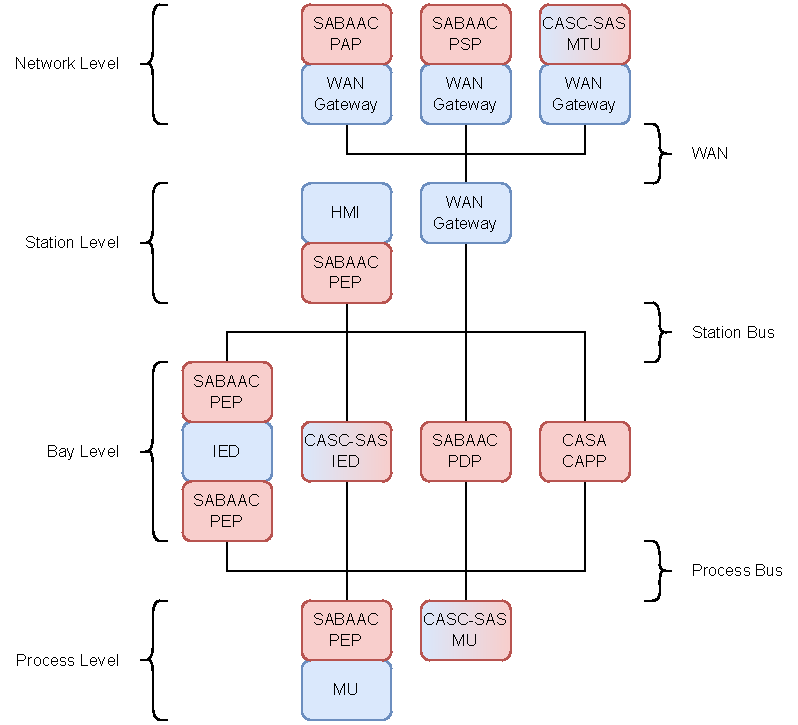
\includegraphics[width=1.0\linewidth]{figures/casc_architecture_color.drawio.pdf}
    \caption{Adaptation of the layered SAS architecture to the CASC-SAS approach.
    % The adaptation of the layered SAS architecture to the CASC-SAS approach entails a modification of the architecture to accommodate the additional components provided by CASC-SAS. The components depicted in blue represent elements of the SAS architecture, whereas the components depicted in red are introduced by the CASC-SAS approach. The components with a color gradient represent elements of the SAS architecture that have been adapted to support CASC-SAS concepts.
    }
    \label{fig:casc_architecture}
\end{figure}

To examine the feasibility and perform the above-mentioned integration, we propose a hardware and software realization of our approach.
The aim of the realization is to provide implementations of CASA and SABAAC with a full range of functions.
The software is going to be implemented component-wise using high-level programming languages.
Depending on the complexity and time constraints of a specific component, different programming languages might be used for the implementation.
Due to internal dependencies, the software implementation is split into two parts.
The first part is dedicated to the CASA approach, as it represents the foundation of all employed protocols.
The second part is dedicated to the SABAAC components and protocols.

The employed components of CASA and SABAAC provide different services.
Furthermore, the components have to be deployed differently to correspond to the proposed protocols.
While PAP and PSP may be deployed centrally, components such as PEP, PDP, UCS, and KGC are distributed to individual SAS instances.
This leads to differing hardware requirements for the implemented components.
Moreover, with the exception of PEP instances, the components provide their services by using a client-server pattern.
The PEP instances partially use a client-server pattern and partially provide their services in the form of a Bump-In-The-Wire (BITW) solution.
The services provided by PEP instances via BITW pattern are automatically applied to captured packets.
Therefore, these services are invisible to the corresponding service consumers.
This BITW pattern is inspired by the security filter approach presented by \citeauthor{Ishchenko2018} \cite{Ishchenko2018}.
Taking the differing provision patterns and deployment structures into account, we propose the usage of performance-oriented server hardware for the PAP, PSP, PDP, UCS, and KGC to avoid bottlenecks and mitigate the risk of accidental or malicious DoS.
Moreover, we propose the usage of inexpensive off-the-shelf hardware for the highly distributed PEP instances.

\section{Evaluation}
\label{sec:approach:evaluation}
In this section, the evaluation of the CASC-SAS approach is discussed.
The goal of the evaluation is to derive quantitative and qualitative characteristics of the approach.
These characteristics are used to verify the applicability of the proposed approach in the presented field of application.
Moreover, the characteristics are used to identify limitations and future work of the proposed approach.

\subsection{Strategy}
The evaluation is performed theoretically as well as experimentally.
For the theoretical parts of the evaluation, formal and informal methods are used to proof certain characteristics of the proposed approach.
The experimentally performed part of the evaluation is based on the realization presented in \autoref{sec:approach:realization}.
The component implementations are used to construct a network simulation and network test bed.
The proposed network test bed is visualized in \autoref{fig:evaluation_test_bed}.
The components depicted in blue represent computers that mimic the behavior of domain-specific senders and receivers of an SAS.
The components depicted in red are part of the CASC-SAS approach.
The components depicted in yellow represent message-forwarding intermediate network devices.

These test environments mimic the behavior of a real interconnected SAS for occurring message exchanges.
The simulation and test bed strategy have differing advantages and disadvantages.
On the one hand, the simulation strategy has the advantage of repeatability and reproducibility due to deterministic behavior, whereas the behavior of the test bed is non-deterministic.
On the other hand, the test bed results are practice-oriented and transferable to the physical SAS domain, whereas the behavior of a real SAS cannot be compared to the deterministic behavior of the network simulation.
\begin{figure}
    \centering
    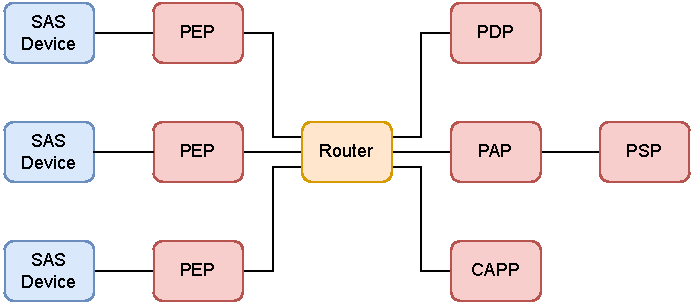
\includegraphics[width=1.0\linewidth]{figures/network_testbed_color.drawio.pdf}
    \caption{Architecture of the network test bed.
    % Architecture of the network test bed used for the experimental evaluation of the CASC-SAS approach. The components depicted in blue represent computers that mimic the behavior of domain-specific senders and receivers of an SAS. The components depicted in red are part of the CASC-SAS approach. The components depicted in yellow represent message-forwarding intermediate network devices.
    }
    \label{fig:evaluation_test_bed}
\end{figure}

\subsection{Evaluation Areas \& Metrics}
The evaluation aims to derive quantitative and qualitative metrics for different areas of interest.
We propose three areas of interest for the evaluation of the CASC-SAS approach.
The three areas of interest and their corresponding metrics are defined as follows:
\begin{description}
    \item[Security Evaluation] Does CASC-SAS provide security against typical SAS adversaries and attacks?
    \begin{enumerate}
        \item Satisfied security, safety, and availability requirements
        \item Assumed system characteristics
        \item Assumed adversary characteristics
        \item Mitigated attacks
        \item Introduced attack surface
    \end{enumerate}
    \item[Performance Evaluation] Is CASC-SAS capable of securing time-constrained communication of an SAS?
    \begin{enumerate}
        \item Satisfied performance requirements
        \item Assumed communication characteristics
        \item Supported message types
        \item Resistance against network exceptions including congestion, delay, jitter, duplicated packets, lost packets, and out-of-order packet delivery
    \end{enumerate}
    \item[Economic Evaluation] Is CASC-SAS an economically feasible solution for the construction or retrofitting of an SAS?
    \begin{enumerate}
        \item Satisfied compatibility requirements
        \item Assumed device requirements
        \item Additional costs for SAS construction and retrofitting
        \item Feasibility with regard to SAS retrofitting
        \item Cost-benefit efficiency compared to alternative approaches
    \end{enumerate}
\end{description}

% \section{Limitations}
% \label{sec:approach:limitations}
% \todo{Reactivate reference in approach introduction}
% \todo{Limitations: No intrusion detection but prevention/mitigation, might not be usable for fast messages, not every crypto for every message type, possible new attack vectors by adding new components, applicability to other ics domains, time protocol interference, physical access control -> future work}
\todo{Section: Limitations}
